\documentclass[twocolumn,a4paper]{article}
\usepackage{graphicx}
\usepackage{subfigure}
\usepackage{amsfonts}
\usepackage{color}
\usepackage{lineno}
\setlength{\columnsep}{10pt}
\setlength{\oddsidemargin}{0pt}
\setlength{\topmargin}{0pt}
\setlength{\headheight}{0pt}
\setlength{\headsep}{0pt}
\setlength{\marginparsep}{0pt}
\setlength{\marginparwidth}{0pt}
\addtolength{\voffset}{-50pt}
\setlength{\textheight}{26.8cm}
\author{Siwang Li}

\title{Material Optimization of a Single Mode}

%% document begin here
\begin{document}
\maketitle

\section{Summary}
For a single mode, it is possible to find the elastic materials by the reduced
displacements. In details, 
\begin{itemize}
\item when there is no damping in generating the input sequence, we
can optimize for $k$ perfectly by using (\ref{qua-en}).
\item when damping is introduced in the input sequence, it is better to optimize
  for both $k$ and the damping $d$ simultaneously(see figure \ref{singleModeKD},
  figure \ref{singleModeD}(a), and residual $E(k,d)$ in table \ref{residual}).
\item even damping is not considered in the optimization(but there is some
  damping in the input animation), the optimized $k$ is also very close to
  $\lambda$(see second experiment and figure \ref{singleModeD}(a)).
\item the initial speed $\dot{z}(0)$ has no impact in the optimization process.
\end{itemize}

\section{Input Animation}
The motion equation of one mode is
\begin{equation} \label{deeq}
  \ddot{z} + (\alpha_m+\alpha_k\lambda)\dot{z} + \lambda z = 0
\end{equation}
and the analytical solution of $z(t)$ is
\begin{equation} \label{oss}
  z(t) = (Pcos(wt) + Qsin(wt))e^{-\alpha t}
\end{equation}
where the angular velocity is defined as $w = \sqrt{\lambda-\alpha^2}$, the
decay rate $\alpha = (\alpha_k\lambda+\alpha_m)/2$, and
\begin{eqnarray}\label{PQ}
  P &=& z(0) \\
  Q &=& \frac{1}{w}(\dot{z}(0) + \alpha z(0))
\end{eqnarray}
We produce the input sequence with a single mode.

\section{Approximate Materials}
Given the input sequence $z_0,\cdots,z_T$, we define a quadratic energy function
\begin{equation} \label{qua-en}
  E(k,d) = \sum_{i=2}^{T-1} \|\frac{1}{h^2}\hat{z}_i+\frac{1}{h}\hat{D}(d)(z_{i+1}-z_{i})+ K(k)z_i\|_2^2
\end{equation}
where $h$ is the time step,$\hat{z}_i=z_{i+1}-2z_{i}+z_{i-1}$,$\hat{D}(d) =
diag(d_1,\dots,d_m)$ is a diagonal matrix represent the damping, and $K(k)$ is a
dense symmetric matrix which is obtained by properly assemble $k_i$ into
$K$. Firstly, we will suppose $\hat{D}$ is known, and optimize for $K$
only. Then we try to optimize for both $K$ and $D$. As we consider only one mode
here, we have $K(k)=k$ and $\hat{D}(d)=d$.

\begin{figure}
  \centering
  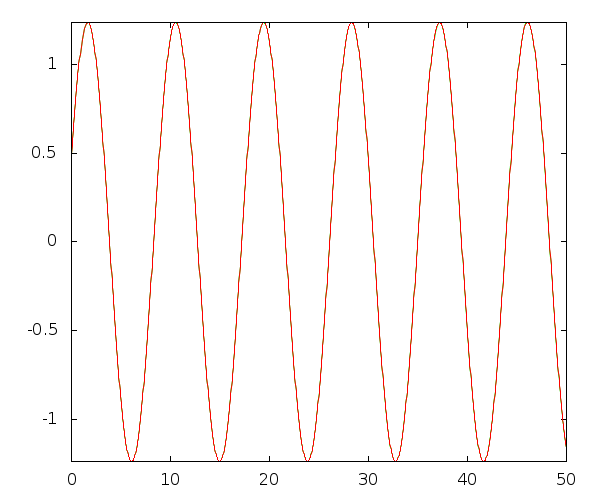
\includegraphics[width=0.4\textwidth]{./figures/singleModeNoDamp.png}
  \caption{Blue is $z(t,\lambda)$, and red is $z(t,k)$, they are overlapped.}
  \label{singleModeNoCon}
\end{figure}
\begin{figure}
  \centering
  \subfigure[$\hat{D}=0$] { \label{fig:a} 
    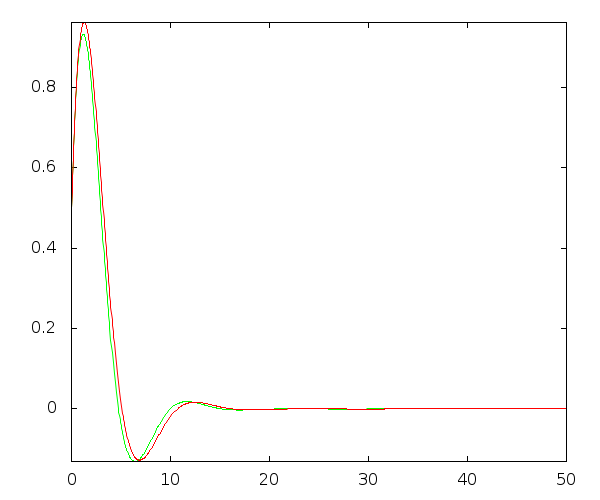
\includegraphics[width=0.4\textwidth]{./figures/singleModeD0.png}
  }
  \subfigure[$\hat{D}=\alpha_k\lambda+\alpha_m$] { \label{fig:b} 
    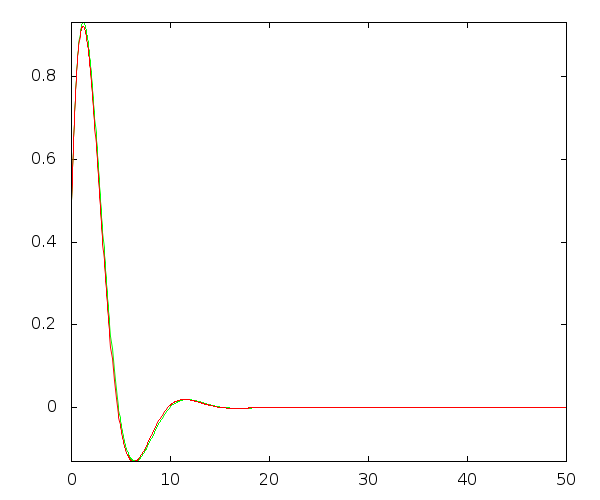
\includegraphics[width=0.4\textwidth]{./figures/singleModeD.png}
  }
  \caption{(a) is $\hat{D}=0$, and (b) is $\hat{D}=\alpha_k\lambda+\alpha_m$ for
    the optimization. In both pictures blue is $z(t,\lambda)$, and red is
    $z(t,k)$.}
  \label{singleModeD}
\end{figure}

\section{Results}
We use a single mode to make the first three experiments, the residuals are
presented at table \ref{residual}.

In the first experiment, we produce the animation of a single mode with
$\lambda=0.5,\alpha_k=\alpha_m=0,T=500,h=0.1,z(0)=0.5,\dot{z}(0)=0.8$. We use
$\lambda$ and $k$ in (\ref{oss}) to obtain two motion curves of $z$, and we
record them as $z(t,\lambda)$ and $z(t,k)$ respectively. We draw curves of these
two functions, and found them almost the same(see figure
\ref{singleModeNoCon}). We also found that the initial speed $\dot{z}(0)$ also
has no impact on fitting $k$.

In the second experiment, we use damping to produce the input animation with
$\alpha_k=\alpha_m=0.5$, and other parameters are same as above. We set
$\hat{D}=0$ and $\hat{D} = \alpha_k\lambda+\alpha_m$ respective to optimize for
$k$. The resulting curves are shown in figure \ref{singleModeD}. It obvious that
when damping are considered in the fitting process, the results will be better.
\begin{figure}
  \centering
  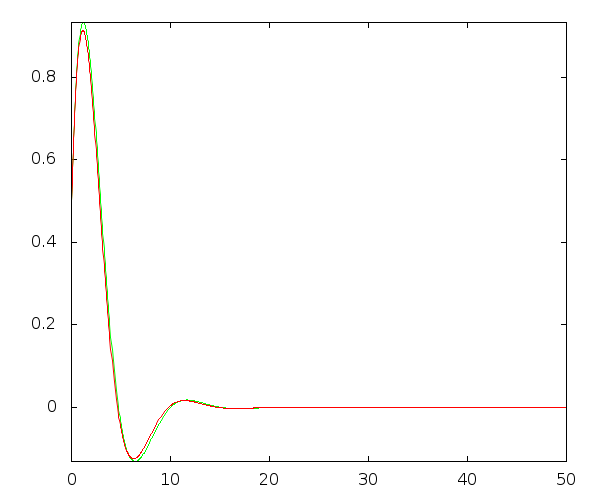
\includegraphics[width=0.4\textwidth]{./figures/singleModeKD.png}
  \caption{blue is $z(t,\lambda)$, and red is new curve with optimized $k$ and
    $d$, e.g $z(t,k,d)$}
  \label{singleModeKD}
\end{figure}

In the third experiment, we use the same setting as above to produce the input
animation, and this time, we optimize for both $d$ and $k$ simultaneously. The
result is shown in figure \ref{singleModeKD}. 

\begin{center}
  \begin{table}[ht]
    {\tiny
      \begin{tabular}{ | l | l | l | l | l| l|}
        \hline
        Figure&$E(k,d)$&$E(\lambda,d')$&$\frac{|k-\lambda|}{\lambda}$&$\frac{|d-d'|}{d'}$\\ \hline
        1&$4\times 10^{-23}$&$1.6\times10^{-5}$&$4.1\times 10^{-4}$&0  \\ \hline
        2(a)&2.63&$2.7$&0.11& 0 \\ \hline
        2(b)&$1.7\times 10^{-3}$&$8.9\times 10^{-3}$&$3.9\times 10^{-2}$& 0 \\
        \hline
        3&$10^{-26}$&$8.9\times 10^{-3}$&$3.8\times 10^{-2}$&$3.8\times 10^{-2}$\\ \hline
      \end{tabular}
}
\caption{The residuals of the experiments of one single mode, where $k$, $d$ is
  the optimized elastic material, while $\lambda$ and
  $d'=\lambda\alpha_k+\alpha_m$ are the corresponding values for generating
  the input animation.} 
\label{residual}
\end{table}
\end{center}

\end{document}
